\documentclass[12pt]{article}
\usepackage[utf8]{inputenc}
\usepackage{graphicx} % For adding images to the document.
\usepackage{calendar} % For timetable object.
\usepackage{multicol} % For multi-column sections.
\usepackage[left=2cm, right=3cm, top=2cm]{geometry} % For setting page margins.
\usepackage{url}
\usepackage{fancyhdr}
\pagestyle{fancy}
\lhead{Kyle Gough}
\usepackage{biblatex}
\addbibresource{references.bib}

\title{CS310 Dissertation\\Using Swarm AI to map a Cave Network}
\author{Kyle Gough}
\date{October 2018}

\begin{document}

\maketitle

\section{Background and Introduction}

Cave exploration is high-effort, time-consuming and potentially dangerous to humans. This is due to such factors as flooding, hypothermia, tight spaces, falling rocks, or harmful gases and particulates such as histoplasmosis from animal droppings \cite{Histoplasmosis}. Some caves in particular are too extensive to fully map and are constantly being further explored which is the case for the Mammoth cave in Kentucky, USA the largest cave network on Earth which contains over 400 miles of cave \cite{Mammoth}. A proposed safer and risk-free method of cave exploration and mapping is to employ a fleet of autonomous flying drones. The drones will use swarm AI to avoid contact with each other and the cavern walls whilst simultaneously identifying potential unexplored paths. The drones will avoid crowding by splitting at junctions to increase exploration efficiency. Communication protocols will be employed to exchange exploration information to minimise mapping duplication and help decide where to explore. Additionally this project is not solely limited to cave exploration, it may be modified to have applications with other real world problems such as: mass deliveries, @@@, @@@, @@@, and @@@.

%OLD: Many unexplored caverns and mine-shafts are dangerous for human exploration due to various factors such as flooding, heat, tight spaces, harmful gases and instability. A safer and risk-free method would be to employ a fleet of autonomous flying drones. The drones will use Swarm AI to avoid contact with each other and the cavern walls whilst simultaneously identifying potential unexplored paths and avoid crowding by splitting up wherever possible to increase the efficiency of the exploration. This project aims to identify and simulate the specific behaviours required to increase the efficiency of cave exploration.

\section{Current Hardware and Software}

\subsection*{Zebedee - CSIRO}
Zebedee is a hand-held device which contains a laser scanner in constant rotation. A human operator holds the device whilst traversing an area and the signals received from the device can be used to create a map of the surrounding area. It allows the creation of a complex and detailed map of the area, however it is restricted by the speed and reachability of the human operator in the environment \cite{Zebedee}. The human operator is at risk of all the dangers of cave exploration.

\pagebreak[4] %###

\subsection*{Hovermap - CSIRO}
Hovermap is an attached to hover drones which uses LIDAR technology to map the entire surrounding environment. It is similar to Zebedee but isn't required to be held and is not restricted by human speed or reach-ability of the environment. The hovermap is not yet capable of interacting with other similar drones to increase exploration efficiency \cite{Hovermap}.

\section{Objectives}

\begin{enumerate}
    \item Create a 2D cave environment generator that is customisable and reproducible. The produced environment should be suitable for simulations to utilise. Some factors of the cave which may wish to be customisable include:
    \begin{list}{$\circ$}{}
        \item Size of open areas.
        \item Size of tunnel areas.
        \item Frequency of open areas.
        \item Total area/volume of open space.
        \item Length of cavern sections.
        \item Stalagmites, stalactites and other natural cave formations.
        \item Cavern wall textures.
    \end{list}
    
    \item Create a simulation of a drone which can:
    \begin{list}{$\circ$}{}
        \item Sense the surrounding environment up to a specific range.
        \item Track its current location and path relative to the starting point.
        \item Locally map and store the currently explored environment.
        \item Sense nearby drones to avoid collisions.
        \item Communicate with nearby drones and exchange exploration information.
        \item Identify possible unexplored areas.
        \item Decide the best path to take to explore an unexplored section.
    \end{list} 
    
    \item Drones should aim to scan the entire cave network. In instances of multiple drones they should work together to map the cave efficiently by:
    \begin{list}{$\circ$}{}
        \item Communicating map information when two drones are in communication distance.
        \item Use exchanged information update the drone's local data.
        \item Explore areas not yet explored by any known drone. Plot an efficient path to these areas.
    \end{list}
    
    \item Drones should aim to follow some rules to avoid unnecessary costs, increase efficiency and improve health and safety. These rules are inspired by a ruleset employed in the 2D simulation BOIDS to steer birds in a flock.
    \begin{list}{$\circ$}{}
        \item Avoid contact with the cave walls and other hazardous environment.
        \item Avoid contact with other drones.
        \item Prioritise areas where other drones are not actively exploring.
        \item Explore areas not yet explored by any known drone.
    \end{list}
    
    \item The final simulation should convey useful information and statistics such as:
    \begin{list}{$\circ$}{}
        \item Total time taken to explore all areas on the cave.
        \item Path taken by each individual drone.
        \item Ratio of explored areas to unexplored areas mapped over time.
        \item Area/Volume of unexplored areas identified by each individual drone.
    \end{list}
    
\end{enumerate}


\section{Possible Extensions}

\begin{itemize}
    \item Be able to generate visualisations and simulate solutions in 3D space.
    \item Use navigation techniques to find the best/safest routes to a specific point in the cave, or from any point in a cave to an exit.
    \item Use machine learning to predict where other drones may have explored in the absence of other drones being nearby to exchange information.
\end{itemize}

\section{Methodology}
An agile approach will allow a simple cave generator to first be implemented, with multiple iterations each including a new feature to the caves such as stalagmites and stalactites. This allows sufficient time to create the drone, swarm and communication behaviours and making it work on a simple cave, then with multiple iterations making it work and be efficient in more complex and realistic cave simulations.

\pagebreak[4]

\section{Testing}
In conjunction with an agile development methodology, test driven development will be used. A test case for each objective will be constructed and then tested to ensure existing code still operates correctly when new features are implemented.
\\\\
The graphical nature of the project will assist in debugging. It will particularly assist in identifying errors in the cave generation algorithms.
\\\\
The effectiveness of the drones' behaviour as a group will be tested against: a single drone working independently, multiple drones working independently without teamwork behaviours and finally different numbers of drones with teamwork behaviour. This will identify how effective the teamwork behaviours are and how the efficiency of cave exploration scales with the number of drones present.


\section{Timetable}

Below is the schedule for the hours per week dedicated to the project. Currently 345 hours have been allocated to the project, exceeding the recommended 300 hours. This is to accommodate any unforeseen circumstances that may occur such as: illness or holidays. A larger workload per week has been allocated to the Christmas break (120 hours) and term 2 (120 hours) because I have 4 modules in term 1 and only 2 modules in term 2. Additionally Easter break is being partially reserved for exam revision.

% \StartingDayNumber=2

% TERM 1 Timetable
\begin{center}
\textsc{\LARGE Term 1} 
\textsc{\large 1st Oct 2018 - 7th Dec 2018}
\end{center}

\begin{calendar}{\textwidth}

\day{}{}
\day{}{}
\day{}{ % Wednesday
12pm-2pm \\[3pt]
2:30pm-4:30pm \\[3pt]
}
\day{}{}
\day{}{ % Friday
2pm-3pm \\[3pt]
}
\day{}{}
\day{}{ % Sunday
12pm-3pm \\[3pt]
}
 
\finishCalendar
\end{calendar}

% XMAS Timetable
\begin{center}
\textsc{\LARGE Christmas} 
\textsc{\large 8th Dec 2018 - 6th Jan 2019}
\end{center}

\begin{calendar}{\textwidth}

\day{}{
12pm-2:30pm \\[3pt]
3pm-5:30pm \\[3pt]
}
\day{}{
12pm-2:30pm \\[3pt]
3pm-5:30pm \\[3pt]
}
\day{}{ 
}
\day{}{
12:00pm-2:30pm \\[3pt]
3:00pm-5:30pm \\[3pt]
}\day{}{
12:00pm-2:30pm \\[3pt]
3:00pm-5:30pm \\[3pt]
}
\day{}{
12:00pm-2:30pm \\[3pt]
3:00pm-5:30pm \\[3pt]
}
\day{}{}
 
\finishCalendar
\end{calendar}

% Term 2 Timetable
\begin{center}
\textsc{\LARGE Term 2} 
\textsc{\large 7th Jan 2019 - 16th Mar 2019}
\end{center}

\begin{calendar}{\textwidth}

\day{}{}
\day{}{}
\day{}{ 
12:00pm-4:00pm \\[3pt]
}
\day{}{}
\day{}{
12:00pm-4:00pm \\[3pt]
}
\day{}{}
\day{}{
12:00pm-4:00pm \\[3pt]
}

 
\finishCalendar
\end{calendar}

% Easter Break Timetable
\begin{center}
\textsc{\LARGE Easter} 
\textsc{\large 17th Mar 2019 - 23rd April 2019}
\end{center}

\begin{calendar}{\textwidth}

\day{}{
12:00pm-2:30pm \\[3pt]
3:00pm-5:30pm \\[3pt]
}
\day{}{ 
}
\day{}{
12:00pm-2:30pm \\[3pt]
3:00pm-5:30pm \\[3pt]
}
\day{}{}
\day{}{
12:00pm-2:30pm \\[3pt]
3:00pm-5:30pm \\[3pt]
}
\day{}{}
\day{}{}
 
\finishCalendar
\end{calendar}

%\begin{multicols*}{2}
\begin{flushleft}

    \begin{itemize}
        \item Term 1 - 1st Oct - 7th Dec
       \begin{list}{$\circ$}{}
            %\item Wednesday 12:00pm-2:00pm, 2:30pm-4:30pm
            %\item Friday 2:00pm-3:00pm
            %\item Sun 12:00pm-3:00pm
            \item \textit{Hours/week: 8, Total Hours: 80}
        \end{list}
        \item Christmas Break - 8th Dec - 6th Jan
         \begin{list}{$\circ$}{}
            %\item Monday 12:00pm-2:30pm, 3:00pm-5:30pm
            %\item Tuesday 12:00pm-2:30pm, 3:00pm-5:30pm
            %\item Thursday 12:00pm-2:30pm, 3:00pm-5:30pm
            %\item Friday 12:00pm-2:30pm, 3:00pm-5:30pm
            %\item Saturday 12:00pm-2:30pm, 3:00pm-5:30pm
            \item \textit{Hours/week: 25, Total Hours: 100}
        \end{list}
        %\vfill\null
        \columnbreak
        \item Term 2 - 7th Jan - 16th Mar
         \begin{list}{$\circ$}{}
            %\item Wednesday 12:00pm-4:00pm
            %\item Friday 12:00pm-4:00pm
            %\item Sunday 12:00pm-4:00pm
            \item \textit{Hours/week: 12, Total Hours: 120}
        \end{list}
        \item Easter Break - 17th Mar - 23rd Apr
         \begin{list}{$\circ$}{}
            %\item Monday 12pm-2:30pm, 3:00pm-5:30pm
            %\item Wednesday 12pm-2:30pm, 3:00pm-5:30pm
            %\item Friday 12pm-2:30pm, 3:00pm-5:30pm
            \item \textit{Hours/week: 15, Total Hours: 45}
        \end{list}
    \end{itemize}

\end{flushleft}
%\end{multicols*}

\pagebreak[4]

The following Gantt chart showcases the different stages of the project and a guideline for when certain deadlines should be met including the design phase, implementation phase which also includes some time for extension work, and the report phase.

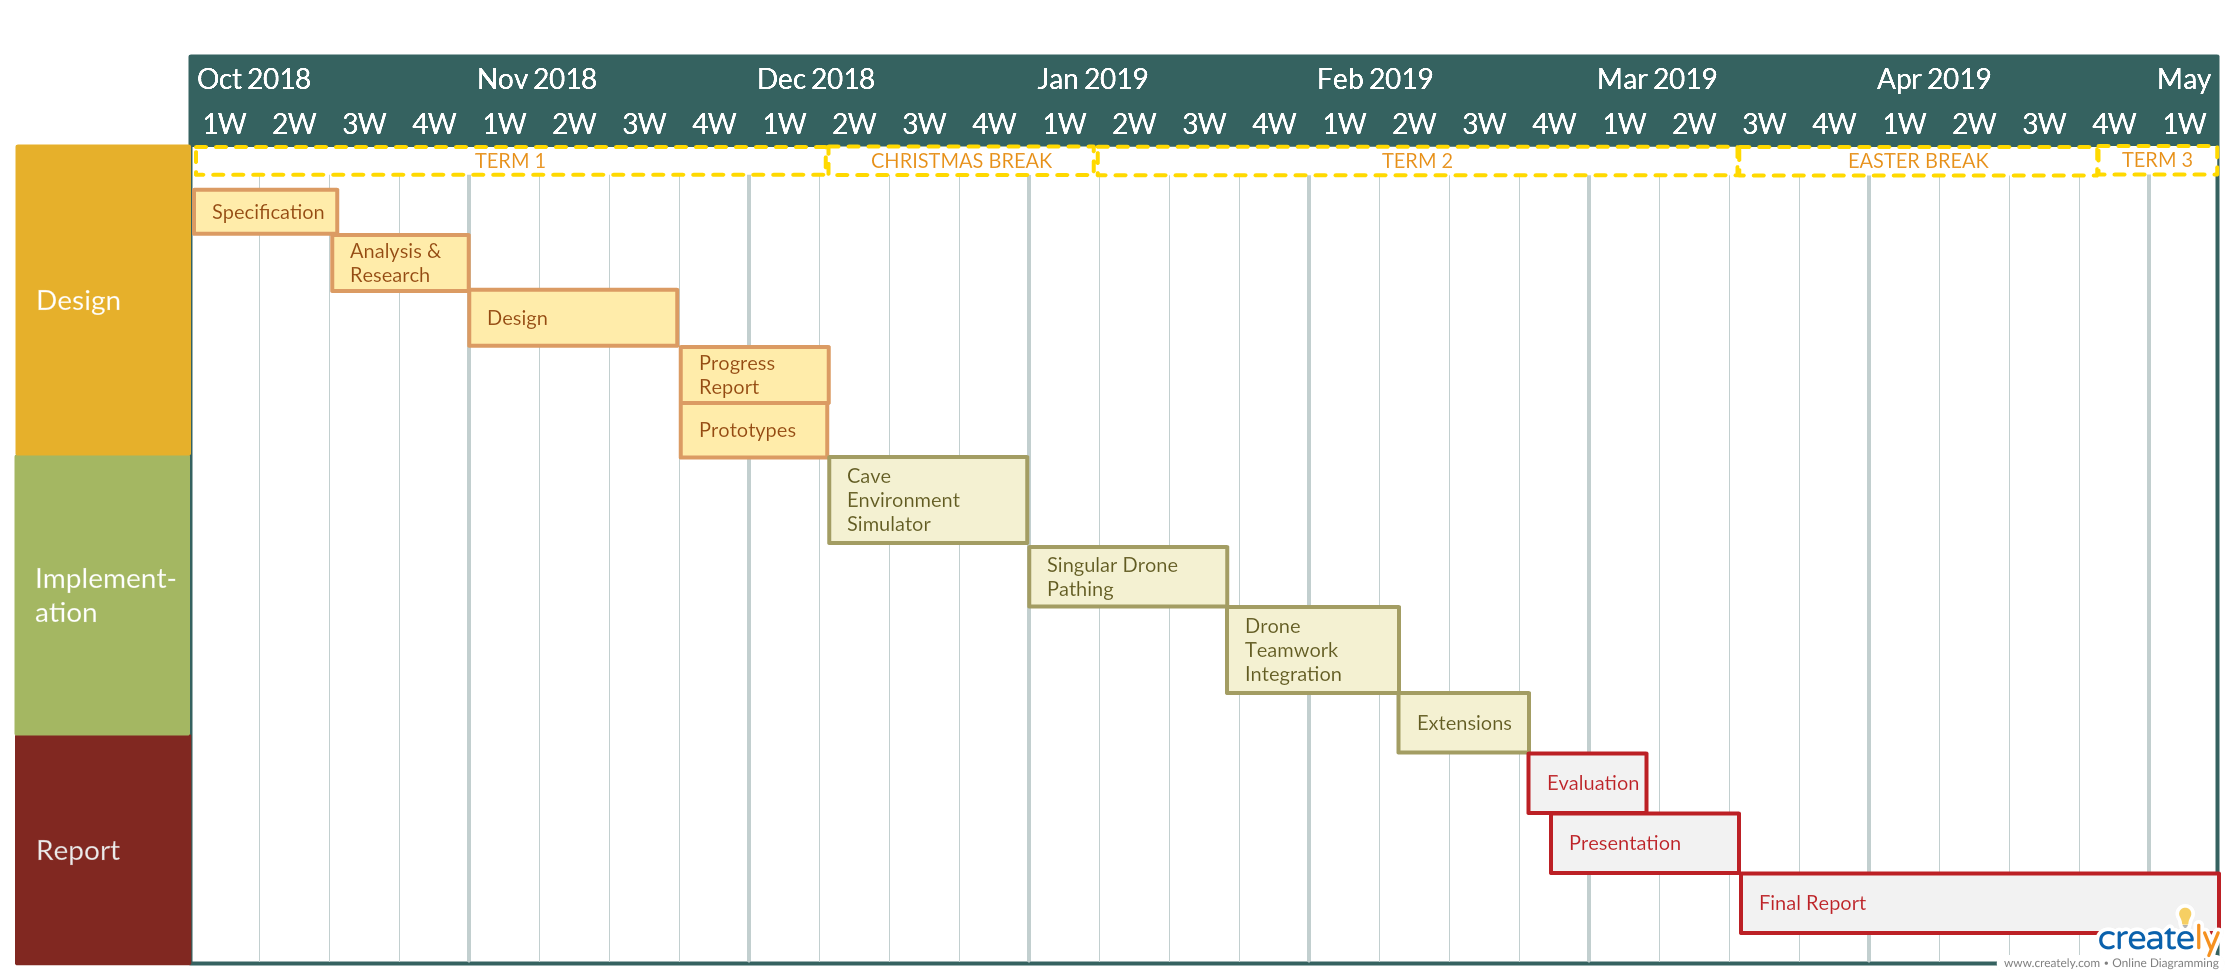
\includegraphics[scale=0.22]{timetable.png}

\section{Risk Assessment}
Here is a list of identified risks and proposed solutions to mitigate them if required.

\begin{itemize}
    \item Risk 1: Illness is a highly potential risk that could occur at any stage of production and can severely slow down progress. Solution 1: Currently the schedule offers more dedicated hours to the project than the recommended amount to account for this risk.
    \item Risk 2: The project is solely dependant on software libraries, and the chosen graphics engine. The risks include the lack of software updates provided by the creator. Using the libraries and engines at a lower version if required will mitigate this risk.
    \item Risk 3: This will be my first project using C++, therefore I may run into errors not yet experienced and will have a slower production rate than other languages I am more familiar with. If the use of C++ becomes too troublesome I can switch to C\# with Unity which I have more familiarity with.
\end{itemize}

\section{Legal, Social and Ethical and Professional Issues}
This project will require no dependencies with other people, therefore there are no issues to consider.

\pagebreak[4]

\section{Resources}

\begin{itemize}
    \item Git - For version control of the software and resources.
    \item Github - For storing the git repository remotely. Provides online version control and backups.
    \item Unity - Game engine with strong graphics capabilities for simulations. For visualisation of the cavern environment and simulating the navigating drones.
    \item C\# - Programming language used in parallel with Unity to create a simulation.
    \item OpenGL - API for 2D and 3D vector graphics. For visualisation of the cavern environment.
    \item C++ - Programming language used in parallel with OpenGL to create a simulation.
\end{itemize}

\printbibliography

\end{document}
